%%=============================================================================
%% Corpus
%%=============================================================================

\chapter{\IfLanguageName{dutch}{Corpus}{Corpus}}
\label{ch:corpus}

\section{Cypress}

Cypress kan geïntegreerd worden in de Visual Studio Code IDE die gebruikt wordt voor Angular development binnen Colruyt Group. Met het commando~\mintinline[breaklines]{bash}{npm install cypress} kan de gebruiker de Cypress software eenvoudigweg installeren. De test cases, alsook het benodigde raamwerk, kunnen vervolgens rechtstreeks in Visual Studio Code geïmplementeerd worden.

\begin{figure}[h!]
    \centering
    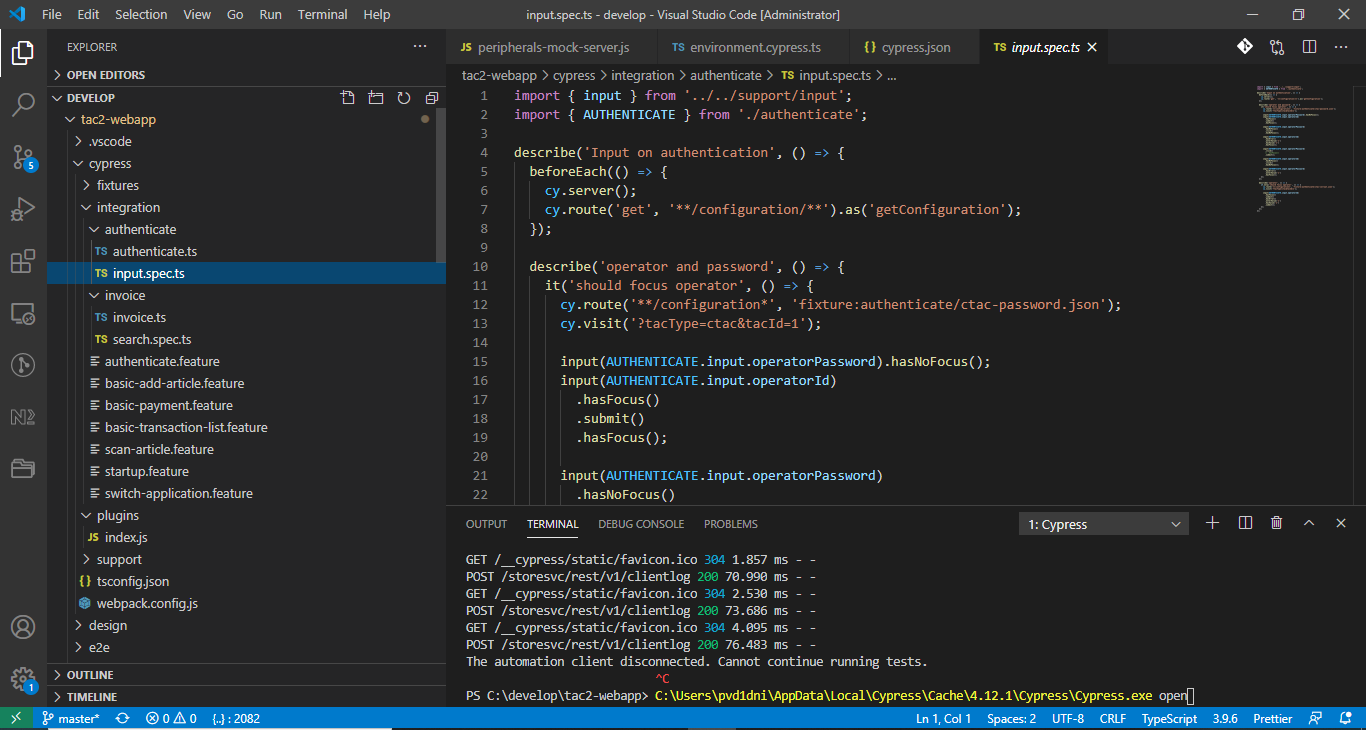
\includegraphics[scale=0.35]{img/corpus/Cypress-In-Visual-Studio.PNG}
    \caption{Cypress in Visual Studio Code}
    \label{fig:CypressInVS}
\end{figure}

De code base voor een test automatisatiesysteem in Cypress wordt in de rootmap van de applicatie geplaatst en bestaat uit 4 belangrijke stukken:

\begin{enumerate}
    \item \emph{Support} — bevat de definities voor alle mogelijke handelingen (``steps''), d.w.z. herbruikbare functies.
    \item \emph{Fixtures} — bevat data-objecten die kunnen gebruikt worden tijdens het mocken van bepaalde services (zoals randapparaten, databanken en externe api's).
    \item \emph{Integration} — bevat de feitelijke tests die gebruik maken van de ``woordenschat'' die gedefiniëerd werd in support.
    \item \emph{Plugins} — eventuele plugins of extensies. In dit onderzoek werd hier geen gebruik van gemaakt.
\end{enumerate}

De randapparaten worden gesimuleerd middels een mock server. Deze server heeft 2 voorname taken:

\begin{enumerate}
    \item Communicaties van de TAC2.0 applicatie naar een randapparaat onderscheppen en een vooraf bepaald antwoord terug sturen. Voorbeelden hiervan zijn: het vrijgeven van de handscanner, het starten van een elektronische betaling op de betaalterminal, en het openen van de geldlade.
    \item Spontane berichten naar de TAC2.0 applicatie sturen, aangestuurd vanuit de testen. Voorbeelden hiervan zijn: ingescande barcodes doorsturen en een wijziging van het gewicht in de weegschaal communiceren.
\end{enumerate}

De code van de mock server kan hieronder gevonden worden.

\begin{minted}[
linenos,
breaklines
]
{JavaScript}
const http = require('http');
const sockjs = require('sockjs');

let sockjs_opts = {
    prefix: '/peripherals',
};

let peripheralsConn;
let sock_peripherals = sockjs.createServer(sockjs_opts);
sock_peripherals.on('connection', function(conn) {
    peripheralsConn = conn;
    console.log('peripherals connection created');
    conn.on('data', function(message) {
        let parsedMessage;
        if (message) {
            parsedMessage = JSON.parse(message);
            console.log('message:', parsedMessage);
            if (parsedMessage.deviceType && parsedMessage.action === 'startup') {
                const output = JSON.stringify({ deviceType: parsedMessage.deviceType, message: 'OK', type: 'STATUS' });
                conn.write(output);
            } else if (parsedMessage.action === 'isScaleEmpty') {
                const output = JSON.stringify({ deviceType: 14, message: 'SCALE_EMPTY', value: '1', type: 'MESSAGE' });
                conn.write(output);
            }
        }
    });
});

const server = http.createServer((request, response) => {
    let bodyChunks = [];
    let message;
    request
    .on('data', (chunk) => {
        bodyChunks.push(chunk);
    })
    .on('end', () => {
        message = Buffer.concat(bodyChunks).toString();
        if (peripheralsConn && message) {
            console.log('Sending message to peripherals websocket');
            peripheralsConn.write(message);
        }
    });
    
    response.end();
});

sock_peripherals.installHandlers(server);

console.log(' [*] Listening on 0.0.0.0:8999');
server.listen(8999, '0.0.0.0');
\end{minted}

De boodschappen die de server moet teruggeven, worden gedefiniëerd in de ``steps''. Onderstaand voorbeeld, te vinden in support\textbackslash step\_definitions\textbackslash peripheral.ts, illustreert de definitie van een ``step'', die zijn argumenten (in dit geval het artikelnummer) meegeeft in een op voorhand bepaald bericht aan de server. De peripherals server zal dit bericht vervolgens naar de TAC2.0 applicatie sturen en simuleert (in dit geval) een bericht dat vanuit de handscanner gestuurd wordt.

\begin{minted}[
linenos,
breaklines
]
{JavaScript}
import { Then } from 'cypress-cucumber-preprocessor/steps';

const peripheralUrl = 'http://localhost:8999/';

Then('I scan article {word}', (articleNr: string) => {
    cy.route('POST', '**/transactions').as('transactionRequest');
    
    const msg = {
        deviceType: 3,
        type: 'MESSAGE',
        message: 'BARCODE',
        value: articleNr,
    };
    
    cy.request(peripheralUrl + 'message', msg);
    cy.wait('@transactionRequest');
});
\end{minted}

Deze ``step'' kan dan gebruikt worden in een ``Feature'', waar de artikelbarcode of het artikelnummer meegegeven wordt als parameter:

\begin{minted}[
linenos,
breaklines
]
{JavaScript}
Feature: Scan an article

@focus
Scenario Outline: I scan an article with the hand scanner
Given Open xtac as <tacType> <tacId> <tacSubType>
When I authenticate as operator <operatorId> and password <password> on "Ctac"
Then Url should be "xtac/ctac/transaction"
When I scan article 5412476144501
And I scan article 5412476042654
Then Url should be "xtac/ctac/transaction/article-details"
And Input <field> should have value <field_value>
And TransactionList row 4 column 2 should look like <column3>
And TransactionList row 4 column 1 should look like <column2>

Examples:
| tacType | tacId | tacSubType | operatorId | password | field            | field_value | column2                    | column3 | subBill           | additionButtons                                 |
| CTAC    |  1    |            | 5          | false    | article_quantity | "1"         | "€ 1,96  \\\| tot: € 1,96" | "1 * 1" | "BUTTON.SUB_BILL" | "BUTTON.SPECIAL_PRICE, BUTTON.PERCENT_DISCOUNT" |
\end{minted}

Als backend van de applicatie werd niet gekozen voor een gemockte backend maar wordt er gebruik gemaakt van een bestaande server die voor pre-productie doeleinden gebruikt wordt. Dit wordt als volgt ingesteld in het environment.cypress.ts bestand dat de omgevingsvariabelen voor Cypress bevat:

\begin{minted}[
linenos,
breaklines
]
{JavaScript}
export const environment = {
    production: false,
    root: '/',
    api: 'http://appserver.colruyt.int/storesvc/rest/v1/', // 'http://localhost:9080/storesvc/rest/v1/',
    ltac: 'http://localhost:9080/ltac',
    peripheralUrl: 'ws://localhost:8999/peripherals/websocket',
    serverMessageUrl: 'ws://localhost:8887',
};
\end{minted}

Deze url wordt vertaald naar het IP-adres van de server in het HOSTS bestand van de computer.

Om de geschreven testen uit te kunnen voeren, dienen 4 processen opgestart te worden vanuit Visual Studio Code:

\begin{enumerate}
    \item Cypress zelf, die vanuit een eerste PowerShell terminal gestart kan worden met het commando~\mintinline[breaklines]{bash}{cypress.exe open}
    \item De TAC2.0 Angular applicatie, die vanuit een tweede PowerShell terminal met de Cypress configuratie gestart wordt:~\mintinline[breaklines]{bash}{ng serve -- configuration=cypress}
    \item Een Node server die randapparaten simuleert, die vanuit een derde PowerShell terminal gestart wordt:~\mintinline[breaklines]{bash}{node server/peripherals-mock-server.js}
    \item Een Chrome browser instantie die door Cypress opgestart wordt bij het lanceren van de testen.
\end{enumerate}

Deze 4 processen worden tijdens uitvoer van de testen gemonitord met de Windows \textsuperscript{\textregistered} Performance Monitor.

\begin{figure}[h!]
    \centering
    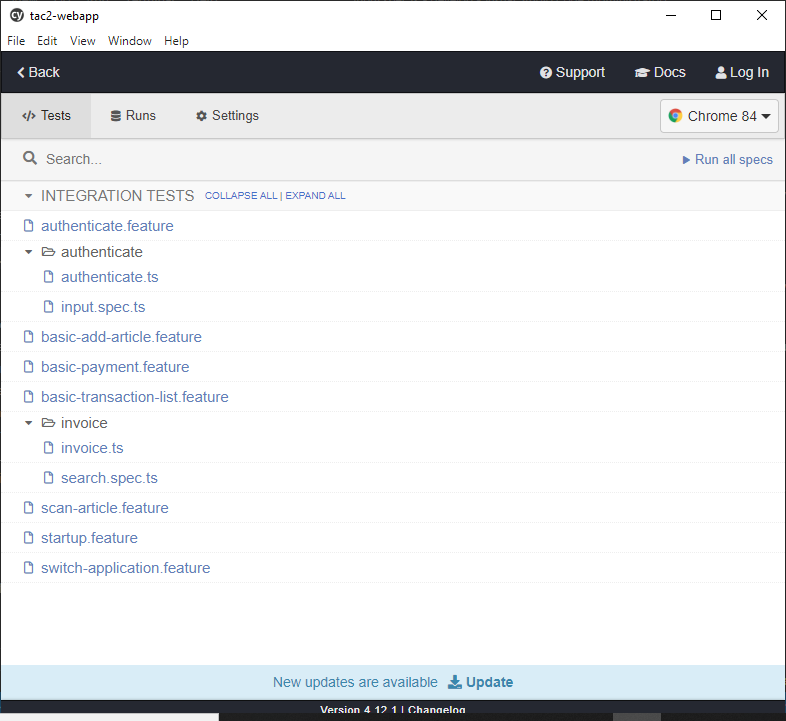
\includegraphics[scale=0.35]{img/corpus/Cypress-UI.PNG}
    \caption{De user interface van Cypress}
    \label{fig:CypressUI}
\end{figure}

\begin{figure}[h!]
    \centering
    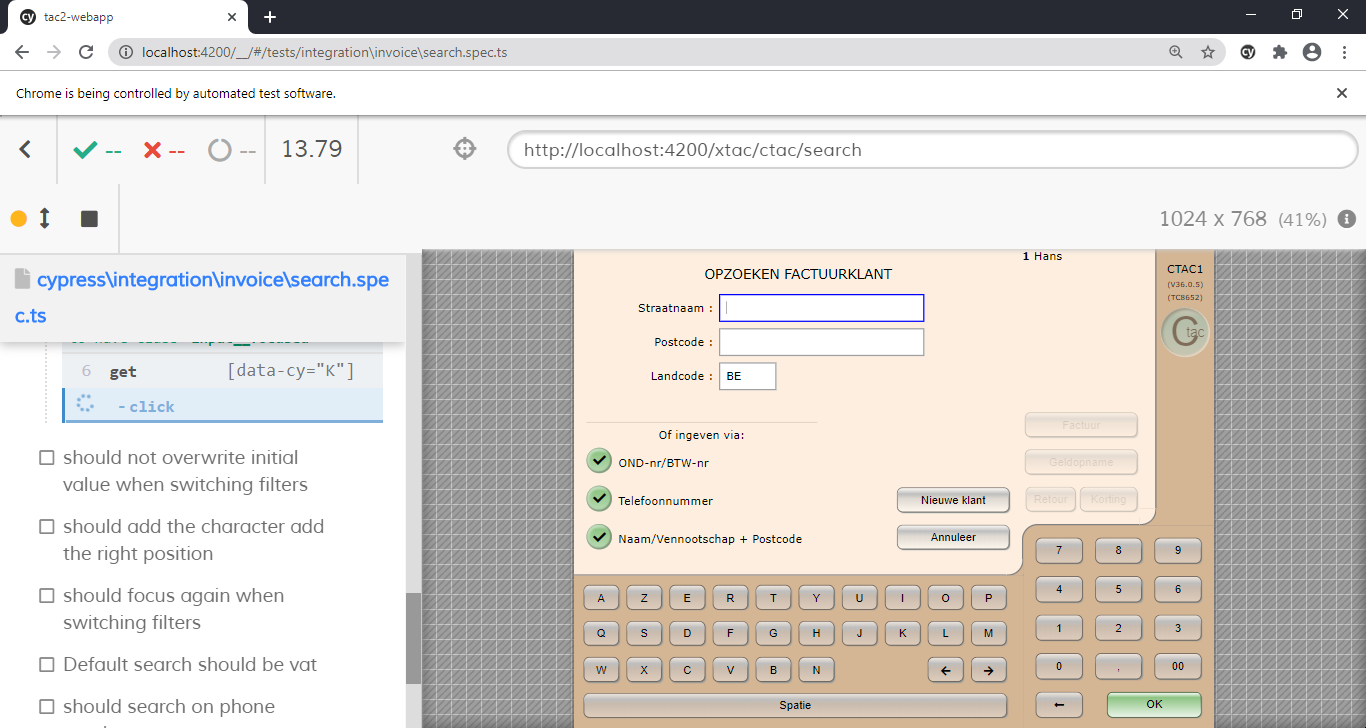
\includegraphics[scale=0.35]{img/corpus/Cypress-Running-Test.PNG}
    \caption{Cypress testen in de Chrome browser}
    \label{fig:CypressRunning}
\end{figure}

%% NB: cypress is vrij beperkt qua mogelijkheden om testen te runnen; je kan via de GUI enkel kiezen om ALLE testen uit te voeren, of om er ÉÉN uit te voeren. Via de command line kan men https://github.com/cypress-io/cypress/issues/3607

\subsection{Requirements}

\textbf{Functionele requirements}:
\begin{itemize}
	\item \textbf{Compatibel met Angular (applicaties)} (MH)
	\begin{itemize}
		\item \emph{Beoordeling}: ja.
	\end{itemize}
	\item \textbf{Compatibel met Chrome} (MH)
	\begin{itemize}
		\item \emph{Beoordeling}: ja.
	\end{itemize}
	\item \textbf{Simulatie van randapparaten} (MH)
	\begin{itemize}
		\item \emph{Beoordeling}: Node server kan gelanceerd worden vanuit Cypress.
	\end{itemize}
	\item \textbf{Auto-synchronisatie} (MH)
	\begin{itemize}
		\item \emph{Beoordeling}: ja.
	\end{itemize}
	\item \textbf{Hergebruik van stappen} (MH)
	\begin{itemize}
		\item \emph{Beoordeling}: ja.
	\end{itemize}
	\item \textbf{Onafhankelijk van andere technologie} (MH)
	\begin{itemize}
		\item \emph{Beoordeling}: ja.
	\end{itemize}
	\item \textbf{Integreerbaar in Visual Studio Code} (NTH)
	\begin{itemize}
		\item \emph{Beoordeling}: ja.
	\end{itemize}
	\item \textbf{Ondersteunt meerdere assertion libraries} (NTH)
	\begin{itemize}
		\item \emph{Beoordeling}: ja.
	\end{itemize}
	\item \textbf{Op Java of JavaScript gebaseerde programmeertaal} (NTH)
	\begin{itemize}
		\item \emph{Beoordeling}: ja.
	\end{itemize}
\end{itemize}

\textbf{Niet-functionele requirements}:
\begin{itemize}
	\item \textbf{Relatief goedkoop} (MH)
	\begin{itemize}
		\item \emph{Beoordeling}: ja, open source.
	\end{itemize}
	\item \textbf{Performant in uitvoer} (MH)
	\begin{itemize}
		\item \emph{Beoordeling}: zie hoofdstuk \ref{ch:verwerking-resultaten}.
	\end{itemize}
	\item \textbf{Vlakke leercurve} (MH)
	\begin{itemize}
		\item \emph{Beoordeling}: Cypress kent geen complexe user interface die men moet leren. Ook is de woordenschat redelijk beperkt en is het dus mogelijk snel met implementaties te beginnen. De features van Cypress zijn daarentegen niet enorm uitgebreid.
	\end{itemize}
	\item \textbf{Toekomstige ondersteuning} (NTH)
	\begin{itemize}
		\item \emph{Beoordeling}: Cypress werd pas in 2018 gereleased, en dit door een relatief klein team. Er bestaat een reëel risico dat dit project in de toekomst \emph{abandonware} wordt.
	\end{itemize}
\end{itemize}

\section{UFT}

In tegenstelling tot Cypress staat UFT volledig los van de ontwikkelomgeving van de applicatie zelf — die vindt namelijk plaats in de alleenstaande Unified Functional Testing applicatie.

\begin{figure}[h!]
    \centering
    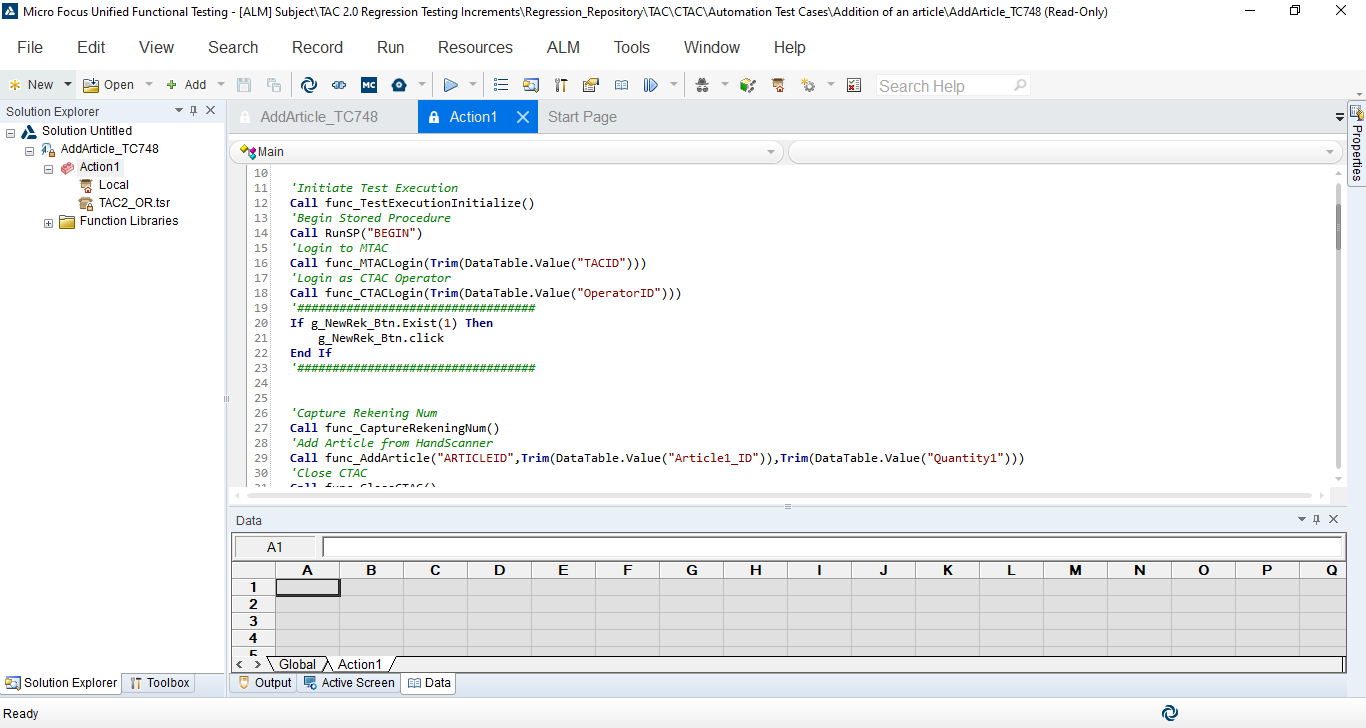
\includegraphics[scale=0.35]{img/corpus/uft-editaction-expertmode.PNG}
    \caption{Het gebruik van expert view in UFT}
    \label{fig:uft-expertview}
\end{figure}

De geautomatiseerde testen in UFT steunen op (grotendeels) dezelfde pijlers als die in Cypress, met enkele verschillen:

\begin{enumerate}
    \item Hoewel testen geschreven worden in UFT, worden de testen gelanceerd vanuit \textbf{HP ALM} (Application Lifecycle Management). Deze applicatie omvat meerdere onderdelen voor het beheren van de levenscyclus van een applicatie, waaronder het \emph{test lab} voor het runnen van zowel geautomatiseerde als manuele testen. De ALM desktop client is beschikbaar vanaf een centrale server en wordt gelanceerd vanuit de browser.
    \item De \textbf{UFT testrunner} is verantwoordelijk voor het uitvoeren en coördineren van de testen en wordt gelanceerd bij het starten van testen vanuit het HP ALM test lab.
    \item UFT heeft een instantie van de \textbf{te testen applicatie} nodig. Hiermee wordt vanuit de testen vervolgens automatisch verbinding gemaakt.
    \item Om de randapparaten te simuleren, wordt voor de testen in UFT gebruik gemaakt van de ``\textbf{peripheral drivers}''. Deze batch-programma's hebben dezelfde functie als de peripherals server die gebruikt werd voor Cypress, met het verschil dat deze een grafische user interface hebben voor elk randapparaat dat gesimuleerd wordt. Deze software wordt ook in de pre-productie omgeving van Colruyt Group gebruikt voor testen op afstand.
\end{enumerate}

\begin{figure}[h!]
    \centering
    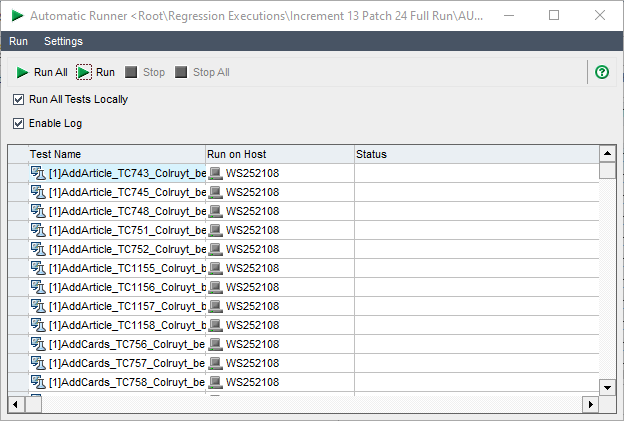
\includegraphics[scale=0.35]{img/corpus/uft-runner.PNG}
    \caption{De UFT testrunner}
    \label{fig:uft-testrunner}
\end{figure}

\begin{figure}[h!]
    \centering
    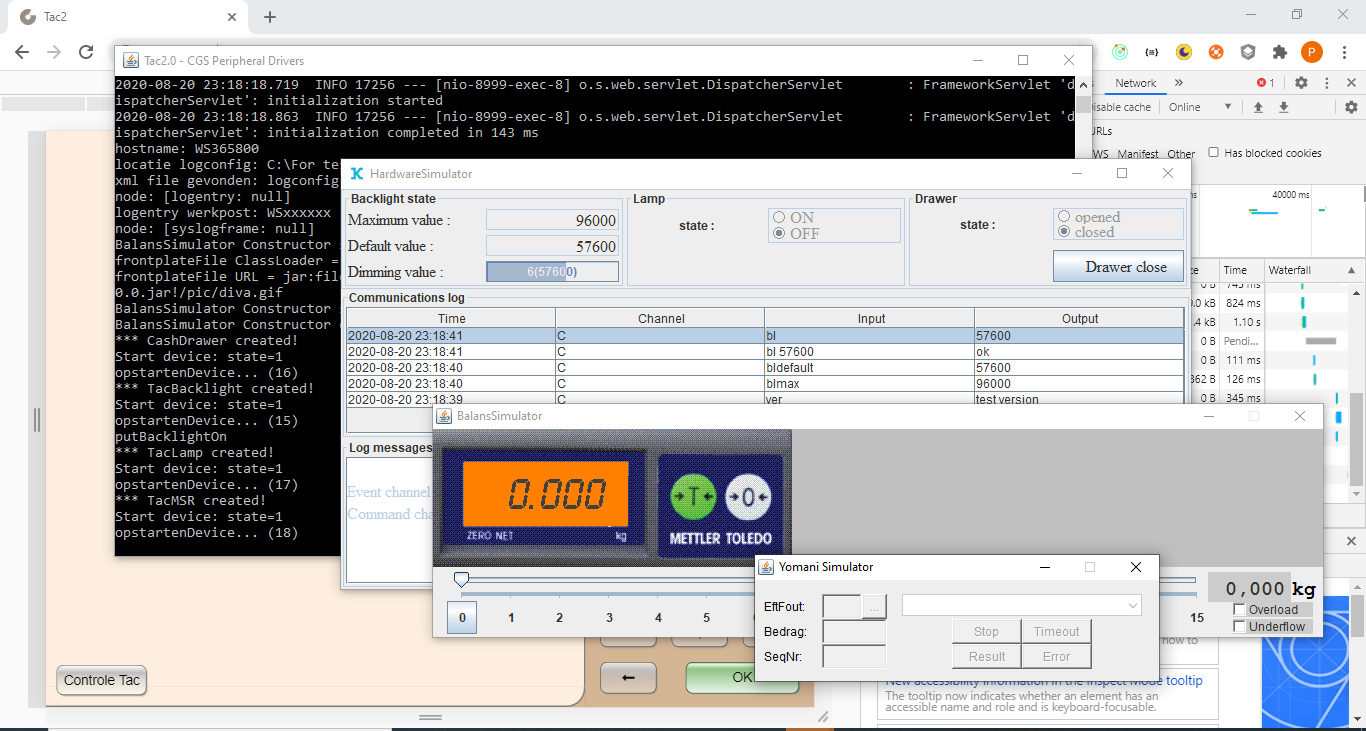
\includegraphics[scale=0.35]{img/corpus/tac20-peripherals.PNG}
    \caption{De grafische peripherals simulator die in pre-productie omgevingen gebruikt wordt binnen Colruyt Group}
    \label{fig:tac2point0-peripherals}
\end{figure}

Zoals Cypress testen in feite ``Features'' zijn die uit ``steps'' bestaan, zo zijn UFT testen een opeenvolging van acties die bestaan uit stappen zoals toegelicht in subsectie \ref{ssec:uft}. Onderstaande functie is daar een goed voorbeeld van. Deze functie — ``AddArticle'' — bevat de nodige logica om een artikel in een bepaalde hoeveelheid toe te voegen aan een rekening. Deze functie interageert rechtstreeks met de objecten van de applicatie, die 

\begin{minted}[
linenos,
breaklines
]
{JavaScript}
Function func_AddArticle(ByVal s_ArticleOrBarCode,ByVal s_ArticleId,ByVal s_Quantity)
   If g_TCExecutionTag=False Then Exit Function
   
   Dim bln_ArtcleID , bln_ManualBarCode , bln_ScanBarCode
   Dim bln_AddArticle , arr_Options , i_ArticleCnt , s_Temp , s_TtlPrice , s_ArtQuantity , s_StukCount
   
   s_ArticleOrBarCode = Replace(s_ArticleOrBarCode," ","")
   s_ArticleId = Trim(s_ArticleId)
   s_Quantity = Trim(s_Quantity)
   If s_ArticleOrBarCode="" OR s_ArticleId="" Then
      Call UpdateReport("User Provided Improper Details for AddArticel. ArticleID/ManualBarcode/ScanBarCode-"&s_ArticleOrBarCode&" ArticleID-"&s_ArticleId&" Quantity-"&s_Quantity,"Fail")
      g_TCExecutionTag=False
      Exit Function
   End If
   
   i_ArticleCnt = UBound(g_ArticleNumArray)
   
   bln_AddArticle = True
   Select Case UCase(s_ArticleOrBarCode)
      Case "ARTICLEID"
         
         If func_ClickObject(g_Artikelnr_Btn) Then
'            If g_ArticleID_Edit.Exist And g_AddArticleClear_Btn.Exist Then
'               Call UpdateReport("Article ID EditBox and Article_Clear Buttons are Available","Pass")
'            ElseIf Not g_ArticleID_Edit.Exist Then
'               Call UpdateReport("ArticleID_EditBox Not-Available","Fail")
'               g_TCExecutionTag=False
'               Exit Function
'            Else
'               Call UpdateReport("Article_Clear Button Not-Available","Fail")
'               g_TCExecutionTag=False
'               Exit Function
'            End If
            '   Add Article ID
            Call func_EnterKeyPadVal(s_ArticleId,g_ArticleID_Edit,"YES")
         Else
            g_TCExecutionTag=False
            Exit Function
         End If
         
      Case "MANUALBARCODE"
'         If Not g_KeyPad_Elm.Exist(1) Then
'            Call UpdateReport("User Unabel to Find KeyPad to Enter Manual-Bar Code","Fail")
'            g_TCExecutionTag=False
'            Exit Function
'         End If
         '   Enter Barcode Manually
         Call func_EnterKeyPadVal(s_ArticleId,g_BarCode_Edit,"YES")

      Case "SCANBARCODE"
         '   Enter Barcode from Hand Scanner
         If Not func_RegisterArtcleFromScanner(s_ArticleId) Then
            g_TCExecutionTag=False
            Exit Function
         End If
         
   End Select
   
   
   If g_Weight = True Or g_BalWeight = True Then
      If g_ArticleWeight_Edit.Exist(1) Then
         If g_TestSetName <> "AUTOMATION_DREAMLAND" Then
            If Trim(g_ArticleWeight_Edit.GetRoProperty("value")) = "0,000" Then
               Call UpdateReport("Weight Value loaded as 0,000 by Default","Done")
            Else
               Call UpdateReport("Weight Value Not-Loaded as 0,000 by Default","Fail")
            End If
         End If
         
         If s_Quantity<>"" Then
            s_Quantity = Replace(s_Quantity,".",",")
'            
            Select Case True
               Case g_Weight
                  Call func_EnterKeyPadVal(s_Quantity,g_ArticleWeight_Edit,"YES")
               Case g_BalWeight   
                  g_ArticleWeight_Edit.Click               
                  Call func_AddWeightInBalSimulator(s_Quantity)
            End Select
            
         Else
            Call UpdateReport("User Provided Empty Value for Article Weight","Fail")
         End If
      Else
         Call UpdateReport("User Unable to find Article Weight EditBox","Fail")
      End If
   ElseIf g_AddArticleQuantity_Edit.Exist(1) Then
         If Trim(g_AddArticleQuantity_Edit.GetRoProperty("value")) = "1" Then
            Call UpdateReport("Weight Value loaded as 1 by Default","Done")
         Else
            Call UpdateReport("Weight Value Not-Loaded as 1 by Default","Fail")
         End If
         If s_Quantity<>"" Then
            If Cint(s_Quantity) <> 1 Then
               Call func_EnterKeyPadVal(s_Quantity,g_AddArticleQuantity_Edit,"YES")
            End If
            
            If (UCase(s_ArticleOrBarCode) = "MANUALBARCODE") AND (Cint(s_Quantity) > 17) Then
               Call func_CheckPopUpAlertAndOptions("Opgelet! Hoeveelheid ="&s_Quantity,"OK---"&g_NotOkText)
'               Call func_SelectPopUpOption("Ok")
               Call func_ClickObject(g_Ok_Selection_Btn)
            End If
         End If
   Else
      Call UpdateReport("User Unable to find Article Quantity EditBox","Fail")
'      End If
   End If
      
   If g_Commerce=UCase("AUTOMATION_COLRUYT_FR") OR UCase(s_Langcode)="F" Then
      Exit Function
   End If      
   If g_EmptyPrice = True Then
      'Enter Unit Price of Article
      If g_ArticleUnitPrice_Edit.Exist(1) Then
         If g_ArticleUnitPrice_Edit.GetRoProperty("disabled")=0 Then
'            Call UpdateReport("User able to Edit Article_Unit_Price EditBox for Central_Price Empty Article","Done")
            g_ArticleUnitPrice_Edit.Click
            If Trim(g_UnitPrice)<>"" Then
               g_ArticleUnitPrice_Edit.Set Trim(g_UnitPrice)
               Call func_ClickObject(g_KeyPad_OK_Btn)
               Call UpdateReport(g_UnitPrice & " value entered in Article_Unit_Price EditBox for Central_Price Empty Article","Done")
            Else
               Call UpdateReport("User Provided Empty value to entered in Article_Unit_Price EditBox for Central_Price Empty Article","Fail")
            End If
'            
         Else
            Call UpdateReport("User unable to Edit Article_Unit_Price EditBox for Central_Price Empty Article","Fail")
         End If
      Else
         Call UpdateReport("User unable to find Article_Unit_Price EditBox for Central_Price Empty Article","Fail")
      End If
   End If
   
   
   If g_DiscountTag = True Then
      If g_DiscountVal <> "" Then
         Call func_AddDiscount(g_DiscountVal)
      Else
         Call UpdateReport("User unable to Empty Value as Discount","Fail")
      End If
   End If
   
   If bln_AddArticle<>True Then
      Call UpdateReport("User unable to Register Article Properly","Fail")
      g_TCExecutionTag = False
      Exit Function
   End If
   
   bln_AddArticle = True
   If Not(i_ArticleCnt = 0 And Trim(g_ArticleNumArray(0))="") Then
      i_ArticleCnt = i_ArticleCnt + 1
   End If
   
   If Not g_Eenheidsprijs_Elm.Exist(1) Then
      Call UpdateReport("User unable to find Eenheidsprijs_Element","Fail")
   End If
   
   
   If Not Browser("Tac2_Browser").Page("Tac2_Page").WebElement("AddingArticle_Elm").WebEdit("ArticleID_Edit").Exist(1) Then
      Call UpdateReport("User unable to find Article Name EditBox","Fail")
      g_TCExecutionTag = False
      Exit Function
   End If
   
   g_NumOfArticles = Cint(g_NumOfArticles) + 1
   If g_NumOfArticles>6 Then
      If g_RekeningTblScrollUp_Btn.Exist Then
         If g_RekeningTblScrollUp_Btn.GetRoProperty("disabled")=0 Then
            Call UpdateReport("ScrollUp Option in Rekening Table is Enabled for "& g_NumOfArticles &" Articles","Pass")
         Else
            Call UpdateReport("ScrollUp Option in Rekening Table is Disabled for "& g_NumOfArticles &" Articles","Fail")
         End If
      Else
         Call UpdateReport("Rekening_Table ScrollUp Button Not Available","Fail")
      End If
   End If

   Select Case Trim(g_TestCaseName)
      Case "AddArticle_TC753","AddArticle_TC754","AddArticle_TC755"
         Call func_CaptureWorkAreaArtDetails(Cint(g_NumOfArticles)-1)
      
   End Select
   Set arr_Options = Nothing
   
   Call func_CheckForOnverwachteFout()
End Function
\end{minted}

De processen die tijdens de praktijktesten gemonitord werden, zijn als volgt: de ALM Client, de HP UFT Chrome Native Messaging Host, de UFT Remote Agent, de Chrome browser, de Batch command terminals die de randapparatensimulatie aansturen en de Java instanties die de GUI van de randapparaten voorzien.

\subsection{Requirements}

\textbf{Functionele requirements}:
\begin{itemize}
	\item \textbf{Compatibel met Angular (applicaties)} (MH)
	\begin{itemize}
		\item \emph{Beoordeling}: ja.
	\end{itemize}
	\item \textbf{Compatibel met Chrome} (MH)
	\begin{itemize}
		\item \emph{Beoordeling}: ja.
	\end{itemize}
	\item \textbf{Simulatie van randapparaten} (MH)
	\begin{itemize}
		\item \emph{Beoordeling}: via externe hulpmiddelen.
	\end{itemize}
	\item \textbf{Auto-synchronisatie} (MH)
	\begin{itemize}
		\item \emph{Beoordeling}: ja.
	\end{itemize}
	\item \textbf{Hergebruik van stappen} (MH)
	\begin{itemize}
		\item \emph{Beoordeling}: ja.
	\end{itemize}
	\item \textbf{Onafhankelijk van andere technologie} (MH)
	\begin{itemize}
		\item \emph{Beoordeling}: ja.
	\end{itemize}
	\item \textbf{Integreerbaar in Visual Studio Code} (NTH)
	\begin{itemize}
		\item \emph{Beoordeling}: neen.
	\end{itemize}
	\item \textbf{Ondersteunt meerdere assertion libraries} (NTH)
	\begin{itemize}
		\item \emph{Beoordeling}: neen.
	\end{itemize}
	\item \textbf{Op Java of JavaScript gebaseerde programmeertaal} (NTH)
	\begin{itemize}
		\item \emph{Beoordeling}: neen, gebruikt VBScript.
	\end{itemize}
\end{itemize}

\textbf{Niet-functionele requirements}:
\begin{itemize}
	\item \textbf{Relatief goedkoop} (MH)
	\begin{itemize}
		\item \emph{Beoordeling}: neen, hoge licentiekosten.
	\end{itemize}
	\item \textbf{Performant in uitvoer} (MH)
	\begin{itemize}
		\item \emph{Beoordeling}: zie hoofdstuk \ref{ch:verwerking-resultaten}.
	\end{itemize}
	\item \textbf{Vlakke leercurve} (MH)
	\begin{itemize}
		\item \emph{Beoordeling}: UFT biedt zowel een keyword view als een expert view. Het programmeren in VBScript kent een redelijk stijle leercurve. Keyword view maakt het ook voor niet-programmeurs mogelijk testen te schrijven, maar ook zij moeten leren werken met het Object Repository. De User Interface van UFT biedt veel functionaliteit, maar is niet vanzelfsprekend.
	\end{itemize}
	\item \textbf{Toekomstige ondersteuning} (NTH)
	\begin{itemize}
		\item \emph{Beoordeling}: UFT (voorheen QTP) bestaat reeds sinds 2001 en is reeds meerdere keren overgekocht. De kans is zeer reëel dat deze oplossing zal blijven bestaan.
	\end{itemize}
\end{itemize}

\section{Protractor}

Omwille van technische uitdagingen en tijdtekort kon Protractor helaas niet in de praktijktesten opgenomen worden.

\subsection{Requirements}

\textbf{Functionele requirements}:
\begin{itemize}
	\item \textbf{Compatibel met Angular (applicaties)} (MH)
	\begin{itemize}
		\item \emph{Beoordeling}: ja.
	\end{itemize}
	\item \textbf{Compatibel met Chrome} (MH)
	\begin{itemize}
		\item \emph{Beoordeling}: ja.
	\end{itemize}
	\item \textbf{Simulatie van randapparaten} (MH)
	\begin{itemize}
		\item \emph{Beoordeling}: neen, het gebruik van een externe tool voor het intercepten en het simuleren van berichten is nodig.
	\end{itemize}
	\item \textbf{Auto-synchronisatie} (MH)
	\begin{itemize}
		\item \emph{Beoordeling}: ja.
	\end{itemize}
	\item \textbf{Hergebruik van stappen} (MH)
	\begin{itemize}
		\item \emph{Beoordeling}: ja.
	\end{itemize}
	\item \textbf{Onafhankelijk van andere technologie} (MH)
	\begin{itemize}
		\item \emph{Beoordeling}: nee, Protractor steunt op Selenium en WebDriver JS.
	\end{itemize}
	\item \textbf{Integreerbaar in Visual Studio Code} (NTH)
	\begin{itemize}
		\item \emph{Beoordeling}: ja.
	\end{itemize}
	\item \textbf{Ondersteunt meerdere assertion libraries} (NTH)
	\begin{itemize}
		\item \emph{Beoordeling}: ja.
	\end{itemize}
	\item \textbf{Op Java of JavaScript gebaseerde programmeertaal} (NTH)
	\begin{itemize}
		\item \emph{Beoordeling}: ja.
	\end{itemize}
\end{itemize}

\begin{figure}[h!]
    \centering
    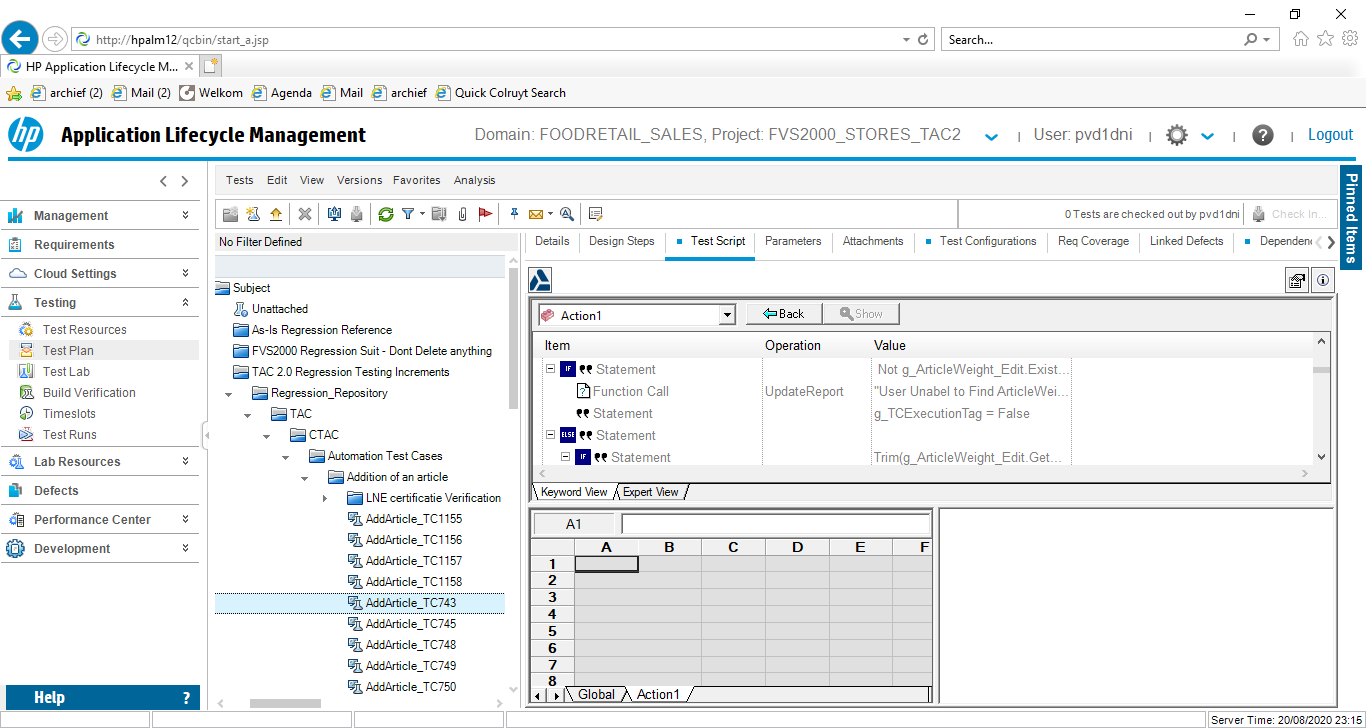
\includegraphics[scale=0.35]{img/corpus/hpalm12-testplan-keywordview.PNG}
    \caption{Het gebruik van de keyword view in HP ALM}
    \label{fig:uft-keywordview}
\end{figure}

\textbf{Niet-functionele requirements}:
\begin{itemize}
	\item \textbf{Relatief goedkoop} (MH)
	\begin{itemize}
		\item \emph{Beoordeling}: ja, open source.
	\end{itemize}
	\item \textbf{Performant in uitvoer} (MH)
	\begin{itemize}
		\item \emph{Beoordeling}: praktijktest niet uitgevoerd.
	\end{itemize}
	\item \textbf{Vlakke leercurve} (MH)
	\begin{itemize}
		\item \emph{Beoordeling}: verschillende bronnen geven aan dat Protractor een vlakke leercurve heeft~\autocite{Mahajan2019, Zavelevsky2014, Enishetti}.
	\end{itemize}
	\item \textbf{Toekomstige ondersteuning} (NTH)
	\begin{itemize}
		\item \emph{Beoordeling}: Protractor wordt ondersteund door Google en bestaat reeds sinds 2013. Er is een zeer reële kans dat Protractor ook in de toekomst zal ondersteund worden, hoewel dit sterk verwoven is met het voortbestaan van Angular zelf.
	\end{itemize}
\end{itemize}